\begin{figure}[ht] 
 	\centering 
 	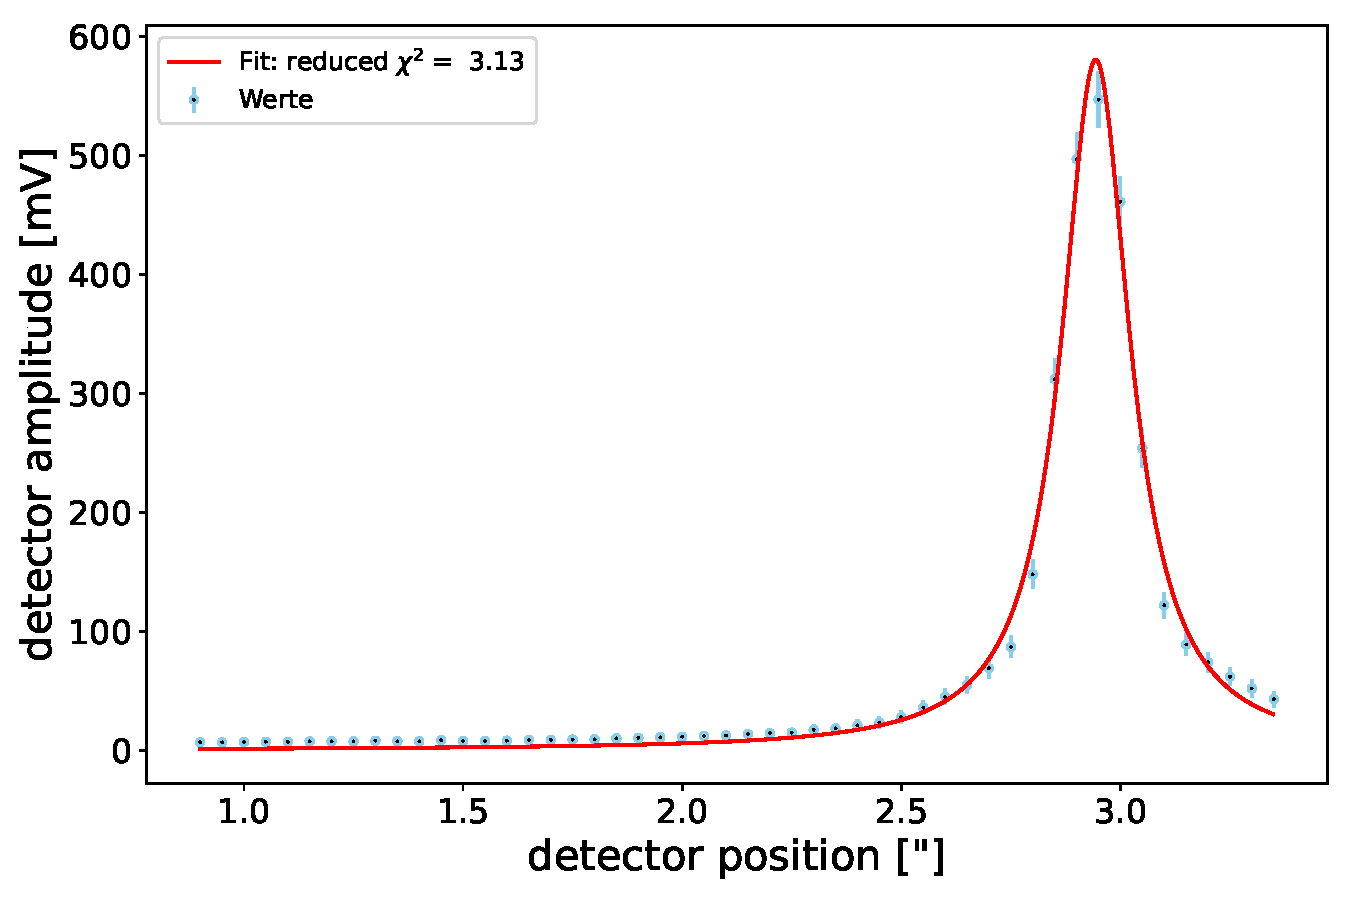
\includegraphics[width= 0.65 \textwidth]{Fits/Amps_B0A_Fit.pdf} 
	\caption{Amps_B0A, Fit} 
 	\label{fig:Amps_B0A, Fit} 
\end{figure}
 \\ 
\begin{table}[ht] 
\centering 
\caption{Amps_B0A, Fit Parameter Tabelle} 
\label{tab:my-table}
\begin{tabular}{|l|c|}
\hline
Parameter Name	&	Wert \\ \hline
amplitude	&	 142.336 \pm  2.926\\ \hline
center	&	 2.943 \pm  0.00191\\ \hline
sigma	&	 0.0542 \pm  0.00134\\ \hline
slope	&	 6.540 \pm  0.955\\ \hline
intercept	&	-2.1286 \pm  1.557\\ \hline
gamma	&	 0.0542 \pm  0.00134\\ \hline
fwhm	&	 0.195 \pm  0.00481\\ \hline
height	&	 548.498 \pm  14.200\\ \hline
\end{tabular} 
\end{table}